\chapter{Diskrete Symmetrien und Erhaltungssätze}
\section{Diskrete Symmetrien}
\begin{figure}
	\centering
	\includegraphics[width=.7\textwidth]{./img/symmetries.jpg}
	\caption{Zusammenfassung der Erhaltungsgrößen}
	\label{fig:symmetries}
\end{figure}

\section{Parität}
\subsection{Der P-Operator}
Der Paritätsoperator $P$ erzeugt eine räumliche Spiegelung im Ursprung.
Sie ist eine mulitplikative Quantenzahl mit den möglichen Eigenwerten $\pm 1$.
Eine Reaktion $a+b\longrightarrow c+d$ hätte die Gesamtparität
\begin{equation*}
	P_a\cdot P_b\cdot (-1)^l = P_c\cdot P_d\cdot (-1)^{l'}
\end{equation*}
mit etwaigen Bahndrehimpulsen $l,l'$.
Dabei sind $P_i$ die \textbf{Eigenparitäten} der Teilchen.
Man definiert:
\begin{align*}
	P(q) &= -P(\bar{q}) = 1 \\
	P(p) &= P(n) = P(\Lambda) = 1
\end{align*}
Außerdem haben bei \textbf{Fermionen} Teilchen und Antiteilchen \textbf{entgegengesetzte} Parität,
bei \textbf{Bosonen} jedoch \textbf{gleiche} Parität.

Alle anderen Paritäten lassen sich daraus ableiten.

\subsection{Paritätsverletzung durch die schwache Wechselwirkung}
Eine einzigartige Eigenschaft der schwachen Wechselwirkung ist die, paritätsverletzend zu sein.
Reaktionen der schwachen Wechselwirkung sind nicht spiegelsymmetrisch.
Dies folgt aus der experimentell belegten Tatsache, dass die schwache Wechselwirkung eine Wechselwirkung mit Axial- und Vektorcharakter zugleich ist.
Die Stärke der Axialvektor- und Vektoranteile werden dabei durch zwei Koeffizienten $c_\text{A}$ und $c_\text{V}$ beschrieben.
Bei einer V+A-Wechselwirkung ($c_\text{V}=c_\text{A}$) koppelt die Wechselwirkung nur an rechtshändige Fermionen und linkshändige Antifermionen.
Bei einer V-A-Wechselwirkung ($c_\text{V}=-c_\text{A}$) koppelt die Wechselwirkung nur an linkshändige Fermionen und rechtshändige Antifermionen.
Für die Kopplungsstärke der W-Bosonen findet man $c_\text{V}=-c_\text{A}=1$.
Man spricht daher auch von einer V-A-Theorie der geladenen Ströme.
Die Parität ist \textbf{maximal verletzt}, wenn gilt: $|c_\text{V}|=|c_\text{A}|$, was bei geladenen Strömen zutrifft.

\begin{figure}
	\centering
	\includegraphics[width=.5\textwidth]{./img/myondecay.pdf}
	\caption{Myonzerfall, eine Möglichkeit ist unterdrückt}
	\label{fig:myondecay}
\end{figure}
Ein Beispiel für die Paritätsverletzung der schwachen Wechselwirkung ist der Myonzerfall $\mu^-\rightarrow\el + \nu_\mu + \bar{\nu}_e$ (\autoref{fig:myondecay}).
Im Ruhesystem des Myons hat das Elektron den größten Impuls, wenn die Impulse der Neutrinos parallel zueinander und entgegengesetzt zur Impulsrichtung des Elektrons stehen.
Da sich die Spins des $\nu\bar{\nu}$-Paares aufheben müssen, muss der Spin des Elektrons dem Spin des Myons gleichgerichtet sein, um Spinerhaltung zu erfüllen.
Experimentell beobachtet man, dass Elektronen aus dem Myonzerfall allerdings bevorzugt linkshändig emittiert werden!
Somit ist die Parität maximal verletzt.

\subsection{Das Wu-Experiment}
\begin{figure}
	\centering
	\begin{subfigure}{0.5\textwidth}
		\centering
		\includegraphics[width=.5\textwidth]{./img/wu.jpg}
		\caption{Das Wu-Experiment: Detektor in negativer z-Richtung}
		\label{fig:wu}
	\end{subfigure}
	\begin{subfigure}{0.4\textwidth}
		\centering
		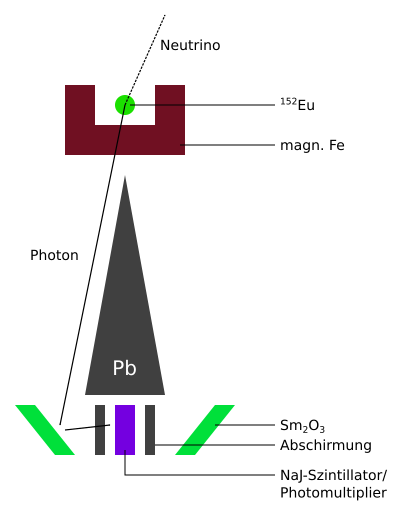
\includegraphics[width=.5\textwidth]{./img/gold.pdf}
		\caption{Das Goldhaber-Experiment: Target unten, Quelle oben}
		\label{fig:gold}
	\end{subfigure}
	\caption{Experimente zur Untersuchung der Paritätsverletzung}
\end{figure}
Eindrucksvoll konnte das Wu-Experiment die Paritätsverletzung der schwachen Wechselwirkung demonstrieren.
Es wurde der Kern-$\upbeta$-Zerfall von $^{60}Co$ untersucht.
Der Versuchsaufbau ist in \autoref{fig:wu} zu sehen.
Die Fragestellung war, ob es eine Vorzugsrichtung der beim $\upbeta$-Zerfall emittierten Elektronen relativ zum Spin des $^{60}Co$-Kerns gibt.
Die Reaktion lautet
\begin{equation*}
	Co(5+)\longrightarrow Ni^*(4+) + \el + \bar{\nu}_e.
\end{equation*}
Die technische Herausforderung dabei war, die Ausrichtung des Spins der Co-Kerne bei sehr tiefen Temperaturen.
Man verwendete das Prinzip der ’’adiabatischen Entmagnetisierung’’ ($\rightarrow$ \url{de.wikipedia.org/wiki/Magnetische_K%C3%BChlung}).

Es wird nun mit einem Detektor in negativer z-Richtung die Anzahl der emittierten Elektronen gemessen, einmal mit Magnetfeld in z-Richtung, einmal in -z-Richtung(, was einer Paritätsumkehr entspricht).
Man stellt fest, dass deutlich mehr Elektronen mit Spin antiparallel zur Spinrichtung der Kerne emittiert werden, als parallel dazu.
Dies ist die Bestätigung der maximalen Paritätsverletzung in der schwachen Wechselwirkung.

\subsection{Das Goldhaber-Experiment}
Das Goldhaber-Experiment zeigt nun sogar, dass es nur linkshändige Neutrinos und rechtshändige Antineutrinos gibt.
Betrachtet wird der Zerfall von Eu-152-Kernen in einem metastabilen Zustand durch K-Einfang
\begin{equation*}
	Eu\text{(meta)} + \el \longrightarrow Sm^* + \nu_e.
\end{equation*}
Der Tochterkern befindet sich in einem angeregten Zustand, der danach durch $\upgamma$-Emission relaxiert.
Dabei erfüllt die Zerfallskaskade folgende Eigenschaften:
\begin{itemize}
	\item Spinfolge $0^-\rightarrow 1^-\rightarrow 0^+$
	\item gleiche Übergangsenergien (ca. 1\% Abweichung der Energien)
	\item Sehr kurze Lebensdauer des Sm ($\approx\SI{3e-14}{\second}$).
\end{itemize}
\autoref{fig:gold} zeigt den Versuchsaufbau.
Der Nachweis der Gamma-Quanten aus dem Sm-Zerfall beruht auf der resonanten Streuung der Gamma-Quanten an einem Sm2O3-Target, welches ringförmig um den Detektor angebracht ist.
Die Bleiabschirmung hindert Zerfallsphotonen aus der Eu-152-Quelle daran, den Detektor direkt zu erreichen.
Die resonante Streuung findet über Kernresonanzabsorption des Photons durch einen Sm-Kern und anschließende spontane Emission statt.
Da die Quellkerne kurze Zeit zuvor ein Neutrino abgegeben haben, ist der angeregte Sm-Kern nicht in Ruhe.
Somit hat das Relaxationsphoton genügend Energie, um resonant absorbiert zu werden und der angeregte Sm-Zustand eine ausreichend geringe Lebensdauer, um nicht durch Wechselwirkungen mit dem Gitter zu relaxieren.
Dieser Trick funktioniert allerdings nur, wenn das Neutrino nach oben emittiert wurde, andernfalls ist die Energiedifferenz zu hoch.
Damit kann also die Richtung der Neutrinoemission bestimmt werden.

Durch einfache Spinbetrachtungen gelangt man zum Schluss, dass die Helizität der Relaxationsphotonen der der emittierten Neutrinos entsprechen muss.
Der Detektor wird von einem magnetisierten Eisenblock abgeschirmt, sodass etwa 7-8\% der Elektronen im Eisen polarisiert sind.
Die Compton-Streuung der Relaxationsphotonen mit den Elektronen im Eisenblock hängt stark von der Polarisierung des streuenden Materials ab.
Falls es eine Vorzugsrichtung der Helizität der Photonen und damit der Neutrinos geben sollte, so müssten sich die Zählraten je nach Magnetisierungsrichtung des Eisenblocks stark unterscheiden.
Tatsächlich misst man nur in eine Magnetisierungsrichtung Ereignisse.

Somit ist bestätigt, dass Neutrinos nur linkshändig vorkommen.

\section{Ladungskonjugation}
\subsection{Der C-Operator}
Der C-Operator führt in einem System Teilchen in Antiteilchen und vice versa über.
\subsection{CP-Erhaltung}
%TODO
TODO
Man kann leicht sehen, dass durch die festgelegte Helizität der Neutrinos die schwache Wechselwirkung C-Symmetrie von vornherein bricht (C auf linkshändiges Neutrino $\rightarrow$ linkshändiges Antineutrino, gibt's aber im SM nicht!).
Wendet man jedoch CP gemeinsam auf Prozesse an, an denen die schwache Wechselwirkung beteiligt ist, so entstehen Prozesse, die in der Natur existieren.
Die schwache Wechselwirkung ist somit CP-erhaltend.
Es gibt jedoch Fälle, bei denen die CP-Symmetrie nicht erhalten bleibt.
